\documentclass[sigconf]{acmart}
\usepackage{amsmath}
\usepackage{amssymb}
\usepackage{csquotes} % displayquote environment
\usepackage{tikz}
\usetikzlibrary{arrows.meta}

\copyrightyear{2019}
\acmYear{2019}
\setcopyright{rightsretained}
\acmConference[]{---}{---}{---}
%\acmBooktitle{}
%\acmPrice{15.00}
%\acmDOI{}
%\acmISBN{}

\begin{document}
\title{Interleaving Anomalies in Collaborative Text Editors}

\author{Martin Kleppmann}
\email{mk428@cl.cam.ac.uk}
\orcid{0000-0001-7252-6958}
\affiliation{%
  \institution{University of Cambridge}
  \streetaddress{William Gates Building, 15 JJ Thomson Avenue}
  \city{Cambridge}
  \state{}
  \postcode{CB3 0FD}
  \country{UK}
}

\author{Victor B.\ F.\ Gomes}
\email{vb358@cl.cam.ac.uk}
\orcid{0000-0002-2954-4648}
\affiliation{%
  \institution{University of Cambridge}
  \streetaddress{William Gates Building, 15 JJ Thomson Avenue}
  \city{Cambridge}
  \state{}
  \postcode{CB3 0FD}
  \country{UK}
}

\author{Dominic P.\ Mulligan}
\email{Dominic.Mulligan@arm.com}
\orcid{0000-0003-4643-3541}
\affiliation{%
  \institution{Arm Research}
  \city{Cambridge}
  \country{UK}
}

\author{Alastair R.\ Beresford}
\email{arb33@cl.cam.ac.uk}
\orcid{0000-0003-0818-6535}
\affiliation{%
  \institution{University of Cambridge}
  \streetaddress{William Gates Building, 15 JJ Thomson Avenue}
  \city{Cambridge}
  \state{}
  \postcode{CB3 0FD}
  \country{UK}
}

\begin{abstract}
  Several published algorithms for collaborative text editing exhibit an undesirable anomaly, in which concurrently inserted portions of text may be interleaved on a character-by-character basis, resulting in an unreadable jumble of letters.
  We highlight algorithms that suffer from this problem, explain its cause, and also identify a lesser variant of the anomaly that occurs in other algorithms.
  Finally, we propose a solution that can, in some cases, prevent the interleaving anomaly.
\end{abstract}

%
% The code below is generated by the tool at http://dl.acm.org/ccs.cfm.
% Please copy and paste the code instead of the example below.
%
\begin{CCSXML}
\end{CCSXML}

\keywords{TODO}
\maketitle

\section{Introduction}

In collaborative software, several users may contribute to a project by creating and editing shared documents, such as text documents, spreadsheets, graphics files, or presentations.
When a user wishes to view a document, a copy of that document is loaded on the user's computer (e.g.\ in a tab of their web browser, or in a native app on their device).
When a user wishes to modify a document, their changes are immediately applied to the copy of the document on the user's computer, and then asynchronously sent to any other users who have a copy of the document (possibly via a server, which may also store a copy).
This collaboration scenario is very similar to the problem of replication in distributed databases: in this context, the shared data is a database rather than a document, and each node that has a copy of the data is called a \emph{replica}.

At a high level, there are two possible ways of managing modifications to documents: either the system enforces that only one user at a time may edit a particular document (for example by obtaining a lock on the file before allowing any modifications), or the system allows multiple users to edit a document concurrently.
The latter case is known as \emph{optimistic replication}.
In an optimistic replication setting, it can happen that several users make changes at the same time, leading the state of these users' documents to diverge.
This is illustrated in Figure~\ref{fig:hello-world}, where one user changes the document \texttt{`Hello!'} to \texttt{`Hello World!'}, while another user concurrently changes it to \texttt{`Hello! :)'}.
In order to ensure that no user input is lost, these concurrent changes must be merged into a consistent document~-- in this example, \texttt{`Hello World! :)'}.

\begin{figure*}[p]
  \centering
  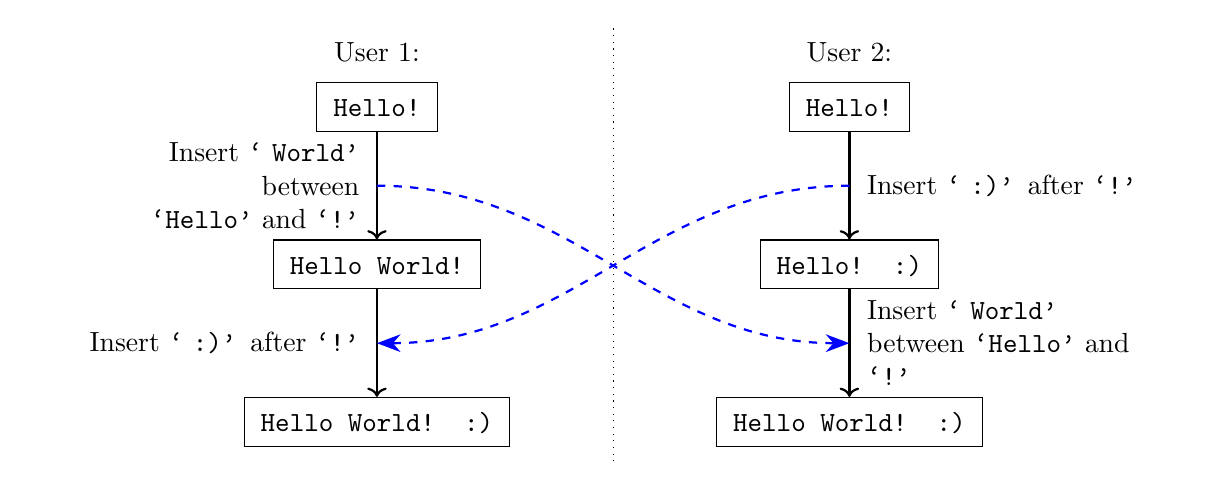
\begin{tikzpicture}[auto,scale=1.0]
    \tikzstyle{box}=[rectangle,draw,inner xsep=6pt,text height=9pt,text depth=2pt]
	\tikzstyle{leftevent}=[left,inner xsep=6pt,text width=4cm,text ragged left,midway]
	\tikzstyle{rightevent}=[right,inner xsep=6pt,text width=4cm,text ragged,midway]
	\tikzstyle{time}=[thick,->]
	\tikzstyle{network}=[thick,dashed,blue,-{Stealth[length=3mm]}]
	\node (left0)  at (0,4.7) {User 1:};
	\node (left1)  at (0,4.0) [box] {\texttt{Hello!}};
	\node (left2)  at (0,2.0) [box] {\texttt{Hello World!}};
	\node (left3)  at (0,0.0) [box] {\texttt{Hello World! :)}};
	\node (right0) at (6,4.7) {User 2:};
	\node (right1) at (6,4.0) [box] {\texttt{Hello!}};
	\node (right2) at (6,2.0) [box] {\texttt{Hello! :)}};
	\node (right3) at (6,0.0) [box] {\texttt{Hello World! :)}};
	\draw [time] (left1)  -- (left2)  node (send1) [leftevent]  {Insert \texttt{`~World'}\\between \texttt{`Hello'} and \texttt{`!'}};
	\draw [time] (right1) -- (right2) node (send2) [rightevent] {Insert \texttt{` :)'} after \texttt{`!'}};
    \draw [time] (left2)  -- (left3)  node (recv2) [leftevent]  {Insert \texttt{` :)'} after \texttt{`!'}};
    \draw [time] (right2) -- (right3) node (recv1) [rightevent] {Insert \texttt{`~World'}\\between \texttt{`Hello'} and \texttt{`!'}};
    \draw [network] (send1.east) to [out=0,in=180] (recv1.west);
    \draw [network] (send2.west) to [out=180,in=0] (recv2.east);
	\path [draw,dotted] (3,-0.5) -- (3,5.0);
  \end{tikzpicture}
  \caption{Simple example of concurrent text editing. Solid black lines indicate state changes over time, while dashed blue arrows indicate network communication.}
  \label{fig:hello-world}
\end{figure*}

\begin{figure*}[p]
  \centering\vspace{2em}
  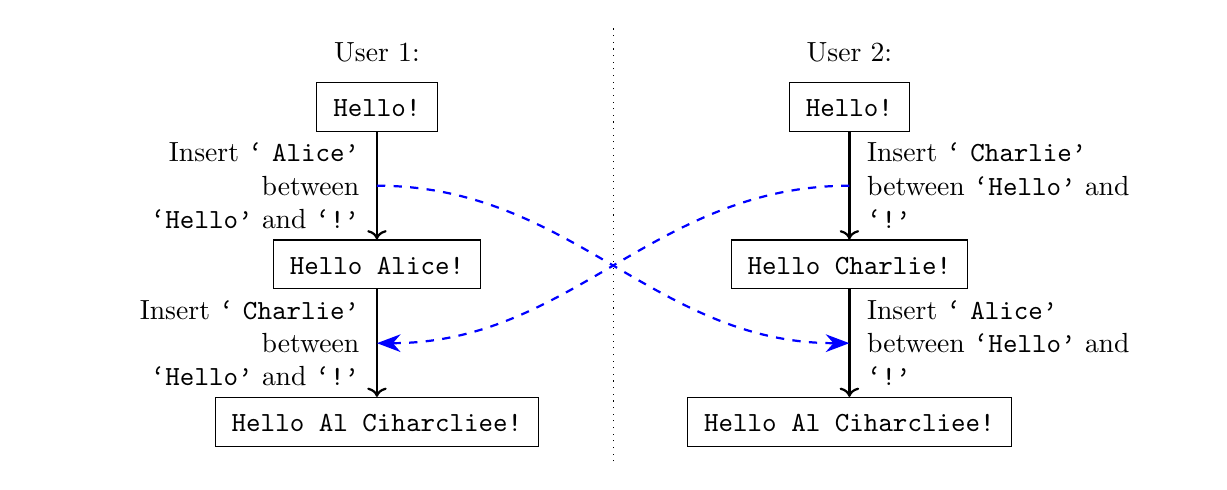
\begin{tikzpicture}[auto,scale=1.0]
    \tikzstyle{box}=[rectangle,draw,inner xsep=6pt,text height=9pt,text depth=2pt]
	\tikzstyle{leftevent}=[left,inner xsep=6pt,text width=4cm,text ragged left,midway]
	\tikzstyle{rightevent}=[right,inner xsep=6pt,text width=4cm,text ragged,midway]
	\tikzstyle{time}=[thick,->]
	\tikzstyle{network}=[thick,dashed,blue,-{Stealth[length=3mm]}]
	\node (left0)  at (0,4.7) {User 1:};
	\node (left1)  at (0,4.0) [box] {\texttt{Hello!}};
	\node (left2)  at (0,2.0) [box] {\texttt{Hello Alice!}};
	\node (left3)  at (0,0.0) [box] {\texttt{Hello Al Ciharcliee!}};
	\node (right0) at (6,4.7) {User 2:};
	\node (right1) at (6,4.0) [box] {\texttt{Hello!}};
	\node (right2) at (6,2.0) [box] {\texttt{Hello Charlie!}};
	\node (right3) at (6,0.0) [box] {\texttt{Hello Al Ciharcliee!}};
	\draw [time] (left1)  -- (left2)  node (send1) [leftevent]  {Insert \texttt{`~Alice'}\\between \texttt{`Hello'} and \texttt{`!'}};
	\draw [time] (right1) -- (right2) node (send2) [rightevent] {Insert \texttt{`~Charlie'}\\between \texttt{`Hello'} and \texttt{`!'}};
    \draw [time] (left2)  -- (left3)  node (recv2) [leftevent]  {Insert \texttt{`~Charlie'}\\between \texttt{`Hello'} and \texttt{`!'}};
    \draw [time] (right2) -- (right3) node (recv1) [rightevent] {Insert \texttt{`~Alice'}\\between \texttt{`Hello'} and \texttt{`!'}};
    \draw [network] (send1.east) to [out=0,in=180] (recv1.west);
    \draw [network] (send2.west) to [out=180,in=0] (recv2.east);
	\path [draw,dotted] (3,-0.5) -- (3,5.0);
  \end{tikzpicture}
  \caption{Two concurrent insertions at the same position are interleaved.}
  \label{fig:bad-merge}
\end{figure*}

\begin{figure*}[p]
  \centering\vspace{2em}
  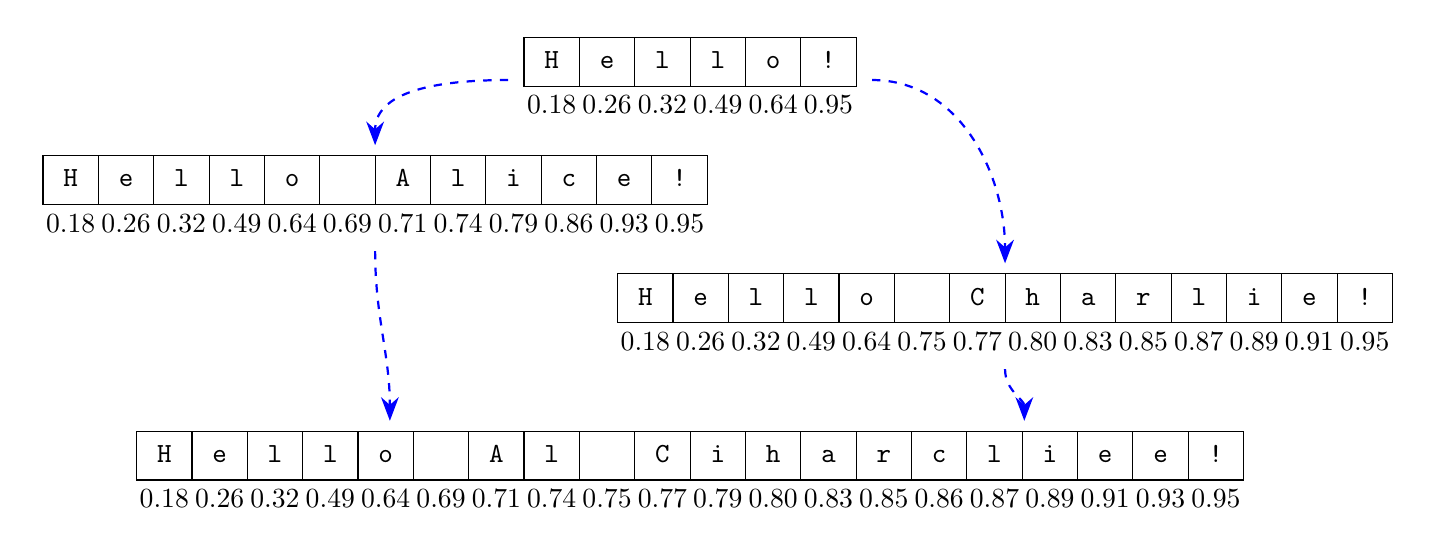
\begin{tikzpicture}[auto,scale=1.0]
    \tikzstyle{box}=[rectangle,draw,inner xsep=6pt,text height=9pt,text depth=2pt]
	\tikzstyle{state}=[matrix,column sep={20pt,between origins}]
	\tikzstyle{val}=[draw,anchor=base,minimum width=20pt,text height=8pt,text depth=3pt]
	\tikzstyle{oid}=[anchor=base]
	\tikzstyle{leftevent}=[left,inner xsep=6pt,text width=4cm,text ragged left,midway]
	\tikzstyle{rightevent}=[right,inner xsep=6pt,text width=4cm,text ragged,midway]
	\tikzstyle{time}=[thick,->]
	\tikzstyle{network}=[thick,dashed,blue,-{Stealth[length=3mm]}]
	\node (hello) at (4,5) [state] {
		\node [val] {\texttt{H}}; &
		\node [val] {\texttt{e}}; &
		\node [val] {\texttt{l}}; &
		\node [val] {\texttt{l}}; &
		\node [val] {\texttt{o}}; &
		\node [val] {\texttt{!}}; \\
		\node [oid] {0.18}; & % H
		\node [oid] {0.26}; & % e
		\node [oid] {0.32}; & % l
		\node [oid] {0.49}; & % l
		\node [oid] {0.64}; & % o
		\node [oid] {0.95}; \\ % !
	};
	\node (alice) at (0,3.5) [state] {
		\node [val] {\texttt{H}}; &
		\node [val] {\texttt{e}}; &
		\node [val] {\texttt{l}}; &
		\node [val] {\texttt{l}}; &
		\node [val] {\texttt{o}}; &
		\node [val] {\texttt{ }}; &
		\node [val] {\texttt{A}}; &
		\node [val] {\texttt{l}}; &
		\node [val] {\texttt{i}}; &
		\node [val] {\texttt{c}}; &
		\node [val] {\texttt{e}}; &
		\node [val] {\texttt{!}}; \\
		\node [oid] {0.18}; & % H
		\node [oid] {0.26}; & % e
		\node [oid] {0.32}; & % l
		\node [oid] {0.49}; & % l
		\node [oid] {0.64}; & % o
		\node [oid] {0.69}; & %
		\node [oid] {0.71}; & % A
		\node [oid] {0.74}; & % l
		\node [oid] {0.79}; & % i
		\node [oid] {0.86}; & % c
		\node [oid] {0.93}; & % e
		\node [oid] {0.95}; \\ % !
	};
	\node (charlie) at (8,2) [state] {
		\node [val] {\texttt{H}}; &
		\node [val] {\texttt{e}}; &
		\node [val] {\texttt{l}}; &
		\node [val] {\texttt{l}}; &
		\node [val] {\texttt{o}}; &
		\node [val] {\texttt{ }}; &
		\node [val] {\texttt{C}}; &
		\node [val] {\texttt{h}}; &
		\node [val] {\texttt{a}}; &
		\node [val] {\texttt{r}}; &
		\node [val] {\texttt{l}}; &
		\node [val] {\texttt{i}}; &
		\node [val] {\texttt{e}}; &
		\node [val] {\texttt{!}}; \\
		\node [oid] {0.18}; & % H
		\node [oid] {0.26}; & % e
		\node [oid] {0.32}; & % l
		\node [oid] {0.49}; & % l
		\node [oid] {0.64}; & % o
		\node [oid] {0.75}; & %
		\node [oid] {0.77}; & % C
		\node [oid] {0.80}; & % h
		\node [oid] {0.83}; & % a
		\node [oid] {0.85}; & % r
		\node [oid] {0.87}; & % l
		\node [oid] {0.89}; & % i
		\node [oid] {0.91}; & % e
		\node [oid] {0.95}; \\ % !
	};
	\node (interleaved) at (4,0) [state] {
		\node [val] {\texttt{H}}; &
		\node [val] {\texttt{e}}; &
		\node [val] {\texttt{l}}; &
		\node [val] {\texttt{l}}; &
		\node [val] {\texttt{o}}; &
		\node [val] {\texttt{ }}; &
		\node [val] {\texttt{A}}; &
		\node [val] {\texttt{l}}; &
		\node [val] {\texttt{ }}; &
		\node [val] {\texttt{C}}; &
		\node [val] {\texttt{i}}; &
		\node [val] {\texttt{h}}; &
		\node [val] {\texttt{a}}; &
		\node [val] {\texttt{r}}; &
		\node [val] {\texttt{c}}; &
		\node [val] {\texttt{l}}; &
		\node [val] {\texttt{i}}; &
		\node [val] {\texttt{e}}; &
		\node [val] {\texttt{e}}; &
		\node [val] {\texttt{!}}; \\
		\node [oid] {0.18}; & % H
		\node [oid] {0.26}; & % e
		\node [oid] {0.32}; & % l
		\node [oid] {0.49}; & % l
		\node [oid] {0.64}; & % o
		\node [oid] {0.69}; & %
		\node [oid] {0.71}; & % A
		\node [oid] {0.74}; & % l
		\node [oid] {0.75}; & %
		\node [oid] {0.77}; & % C
		\node [oid] {0.79}; & % i
		\node [oid] {0.80}; & % h
		\node [oid] {0.83}; & % a
		\node [oid] {0.85}; & % r
		\node [oid] {0.86}; & % c
		\node [oid] {0.87}; & % l
		\node [oid] {0.89}; & % i
		\node [oid] {0.91}; & % e
		\node [oid] {0.93}; & % e
		\node [oid] {0.95}; \\ % !
	};
	\draw [network] (hello.west)    to [out=180,in=90] (alice.north);
	\draw [network] (hello.east)    to [out=0,in=90]   (charlie.north);
	\draw [network] (alice.south)   to [out=270,in=90] (interleaved.170);
	\draw [network] (charlie.south) to [out=270,in=90] (interleaved.9);
  \end{tikzpicture}
  \caption{Interleaving occurs because characters are assigned positions in a dense identifier space, e.g.\ the real numbers $\mathbb{R}$.}
  \label{fig:real-numbers}
\end{figure*}

This kind of merge can either be performed manually (the approach employed by most version control systems, such as git), or it can be automated.
Conflict-free Replicated Data Types, or CRDTs~\cite{Shapiro:2011wy,Shapiro:2011un}, have been developed to automate such merges.
A CRDT is an abstract datatype whose state can be modified by performing certain operations (for example, a datatype for text editing may allow characters to be inserted or deleted anywhere in the document).
It allows arbitrary operations to be performed on different replicas; either the updated state or the operations are then sent over the network and applied or merged into copies of the document on other replicas.

\subsection{Consistency for Optimistic Replication}

CRDTs implement a consistency model called \emph{strong eventual consistency}~\cite{Shapiro:2011un,Gomes:2017gy}, which is defined by the following properties:
\begin{description}
\item[Eventual delivery:] An update applied on one correct replica is eventually applied on all correct replicas.
\item[Convergence:] If the same set of updates have been applied on two replicas, those replicas have equivalent state.
\item[Termination:] All method executions terminate.
\end{description}
In operation-based CRDTs the convergence property is implemented by ensuring that concurrent operations commute.
For example, in Figure~\ref{fig:hello-world}, User 1 first applies the insertion of \texttt{` World'} and then the insertion of \texttt{` :)'}, while User 2 applies the insertions in the opposite order.
Commutativity of the insertions ensures that the outcome is the same in both cases.

When replicas mutually merge each others' changes, the convergence property ensures that those replicas end up in the same state.
However, nothing so far has specified what that state should be.
This means that, although strong eventual consistency is necessary, it is not sufficient, as it does not capture all of the consistency properties that we require in a collaborative application.

In this paper we examine a particular consistency property for collaborative text editors that has so far been overlooked in the literature.
A failure to satisfy this property may result in arbitrary text interleaving, potentially resulting in an undesirable document state.
We highlight existing CRDT algorithms and a specification that exhibit this anomaly, and compare them to other approaches that do not suffer from this anomaly, or only a lesser variant.


\section{The Interleaving Anomaly}\label{sec:anomaly}

Several CRDTs for text documents have been developed, including RGA \cite{Roh:2011dw}, Treedoc \cite{Preguica:2009fz}, WOOT \cite{Oster:2006wj}, Logoot \cite{Weiss:2009ht,Weiss:2010hx}, and LSEQ \cite{Nedelec:2013ky,Nedelec:2016eo}.
In this section we show that two of these algorithms, Logoot and LSEQ, suffer from an anomaly that can lead to undesirable outcomes in some collaborative editing scenarios.
In prior work~\cite{ExtendedVersion,AFP} we proved formally that RGA does not suffer from this problem; however, RGA can exhibit a lesser variant of the anomaly, which we describe in Section~\ref{sec:lesser}.
We conjecture that Treedoc and WOOT do not suffer from either anomaly, but we leave a rigorous proof of this claim for future work.

The anomaly arises when two users concurrently insert text at the same position in a document.
For example, in Figure~\ref{fig:bad-merge}, two users are editing a text document that initially reads \texttt{`Hello!'}.
User 1 changes it to read \texttt{`Hello Alice!'}, while concurrently User 2 changes it to \texttt{`Hello Charlie!'}.
However, when the concurrent edits are merged, the algorithm randomly interleaves the two insertions of \texttt{`~Alice'} and \texttt{`~Charlie'} character by character, resulting in an unreadable jumble of characters.

The reason why this anomaly occurs with Logoot and LSEQ is illustrated in Figure~\ref{fig:real-numbers}.
Conceptually, these algorithms work by assigning every character of the text a unique position identifier from a \emph{dense} space; that is, for any two given identifiers we can create a new, distinct identifier that lies between the two.
The order of characters in the text is then given by the order of these identifiers.
In Figure~\ref{fig:real-numbers} we use real numbers between 0.0 and 1.0 as identifiers (in reality, identifiers in Logoot and LSEQ are paths through a tree, but the effect is equivalent).

We can see in Figure~\ref{fig:real-numbers} that identifiers are assigned correctly by each of the users: the characters of \texttt{` Alice'} and \texttt{` Charlie'} are all assigned numbers between 0.64 and 0.95 (the identifier interval between the preceding \texttt{`Hello'} and the following \texttt{`!'}), in increasing order.
However, the exact values assigned to each character vary randomly, and since neither user knows about the other user's concurrent insertion, both users spread the identifiers of their insertions across the interval (0.64, 0.95).
When merged, the resulting character sequence is a random interleaving of the two insertions.

We performed tests with open source implementations of Logoot \cite{AhmedNacer:2011ke,ReplicationBenchmark} and LSEQ \cite{LSEQTree,Nedelec:2016eo}, and observed this interleaving anomaly occurring in practice.
The problem is even worse if the concurrent insertions are not just a single word, but an entire paragraph or section.
In these cases, interleaving the users' insertions would most likely result in an entirely incomprehensible text that would have to be deleted and rewritten.
Even though the merge in Figure~\ref{fig:bad-merge} is so obviously undesirable, to our knowledge our work~\cite{ExtendedVersion} was the first to point out this anomaly.

This problem does not occur in the example of Figure~\ref{fig:hello-world}.
Here, the merged outcome is unambiguous because the relative ordering of all parts of the text is clear: \texttt{` World'} is inserted before the exclamation mark, while the \texttt{` :)'} is inserted after it.

\subsection{Attiya et al.'s Specification}\label{sec:attiya-spec}

In 2016, Attiya et al.~\cite{Attiya:2016kh} proposed $\mathcal{A}_\textsf{strong}$, an implementation-independent specification of collaborative text editing.
However, this specification also allows the interleaving anomaly.
The definition of $\mathcal{A}_\textsf{strong}$ is as follows~\cite{Attiya:2016kh}:

\begin{displayquote}
  An abstract execution $A = (H, \textsf{vis})$ belongs to the \emph{strong list specification} $\mathcal{A}_\textsf{strong}$ if and only if there is a relation $\textsf{lo} \subseteq \textsf{elems}(A) \times \textsf{elems}(A)$, called the \emph{list order}, such that:
  \begin{enumerate}
    \item Each event $e = \mathit{do}(\mathit{op}, w) \in H$ returns a sequence of elements $w=a_0 \dots a_{n-1}$, where $a_i \in \textsf{elems}(A)$, such that
    \begin{enumerate}
      \item $w$ contains exactly the elements visible to $e$ that have been inserted, but not deleted:
	    \begin{align*}
          \quad\forall a.\; a \in w \quad\Longleftrightarrow\quad &
		  (\mathit{do}(\textsf{ins}(a, \_), \_) \le_\textsf{vis} e) \;\wedge\\ &
		  \neg(\mathit{do}(\textsf{del}(a), \_) \le_\textsf{vis} e).
		\end{align*}
      \item The order of the elements is consistent with the list order:
        \[ \forall i, j.\; (i < j) \;\Longrightarrow\; (a_i, a_j) \in \textsf{lo}. \]
      \item Elements are inserted at the specified position:
        if $\mathit{op} = \textsf{ins}(a, k)$, then $a = a_{\mathrm{min} \{k,\; n-1\}}$.
    \end{enumerate}
    \item The list order $\textsf{lo}$ is transitive, irreflexive and total, and thus determines the order of all insert operations in the execution.
  \end{enumerate}
\end{displayquote}
It is easy to see that the list order relation $\textsf{lo}$ plays the same role as the position identifiers in Figure~\ref{fig:real-numbers}, and hence that this specification allows the same interleaving anomaly.
We can correct this flaw in the $\mathcal{A}_\textsf{strong}$ specification and rule out interleaving by introducing an additional clause 1(d):

\begin{enumerate}
  \item Each event $e = \mathit{do}(\mathit{op}, w) \in H$ returns a sequence of elements $w=a_0 \dots a_{n-1}$, where $a_i \in \textsf{elems}(A)$, such that
  \begin{enumerate}
    \item \dots~(c): as before;
    \setcounter{enumii}{3}
    \item Concurrent insertions are not interleaved: that is, for any two sets of insertions $X$ and $Y$
      \begin{align*}
        X = \{x \mid \exists a.\; &x = \mathit{do}(\textsf{ins}(a, \_), \_) \,\wedge\, x \le_\textsf{vis} e\}\\
        Y = \{y \mid \exists a.\; &y = \mathit{do}(\textsf{ins}(a, \_), \_) \,\wedge\, y \le_\textsf{vis} e\}
      \end{align*}
      such that all operations in $X$ and $Y$ are concurrent:
      \[ \forall x \in X.\; \forall y \in Y.\; \neg(x \le_\textsf{vis} y) \wedge \neg(y \le_\textsf{vis} x) \]
      if the insertions are at the same location in the document:
      \[ \exists i,j.\; \{a_k \mid i < k < j\} = \{a \mid \mathit{do}(\textsf{ins}(a, \_), \_) \in X \cup Y\} \]
      then we have either
      \begin{align*}
        \forall i, j.\; & \mathit{do}(\textsf{ins}(a_i, \_), \_) \in X \;\wedge\; \mathit{do}(\textsf{ins}(a_j, \_), \_) \in Y\\
        & \Longrightarrow\; i < j \quad\text{or}\\
        \forall i, j.\; & \mathit{do}(\textsf{ins}(a_i, \_), \_) \in X \;\wedge\; \mathit{do}(\textsf{ins}(a_j, \_), \_) \in Y\\
        & \Longrightarrow\; j < i.
      \end{align*}
      That is, either all $X$ insertions appear before all $Y$ insertions in the document $w=a_0 \dots a_{n-1}$, or vice versa, but they are never interleaved.
  \end{enumerate}
  \item as before.
\end{enumerate}

\begin{figure*}
  \centering
  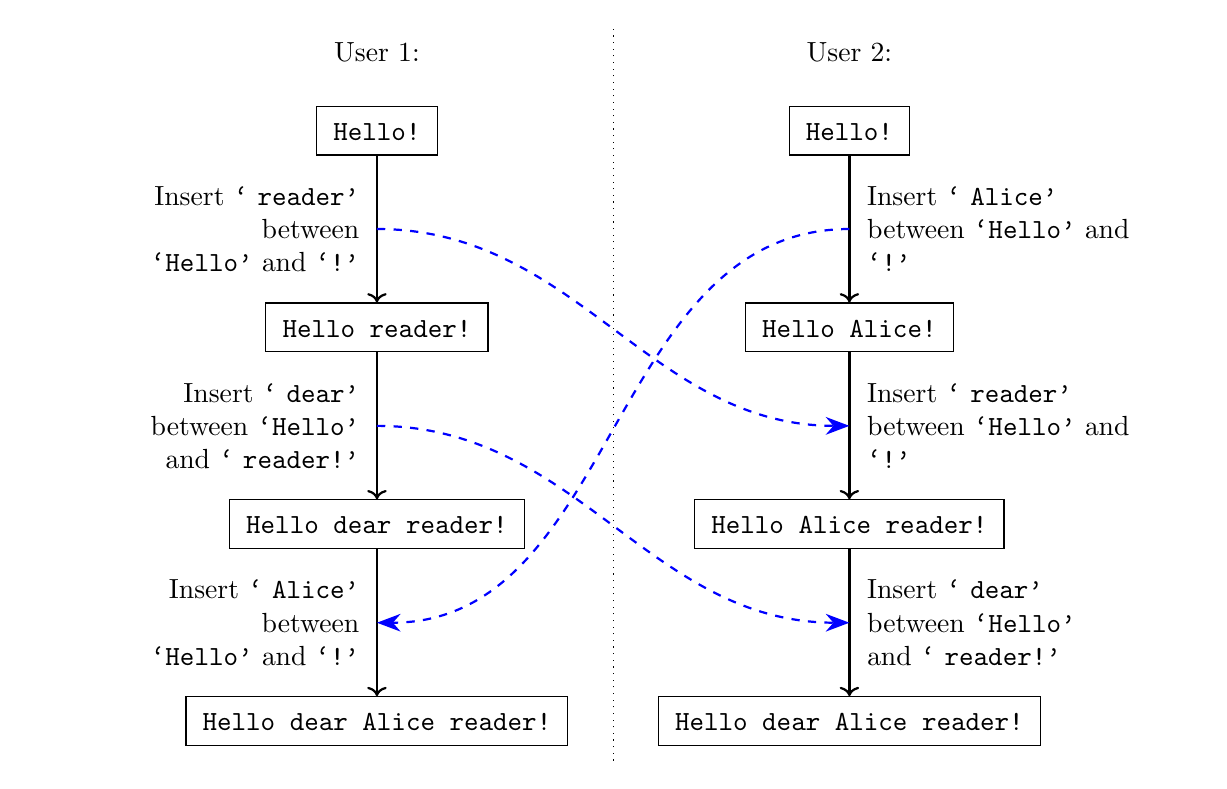
\begin{tikzpicture}[auto,scale=1.0]
    \tikzstyle{box}=[rectangle,draw,inner xsep=6pt,text height=9pt,text depth=2pt]
	\tikzstyle{leftevent}=[left,inner xsep=6pt,text width=4cm,text ragged left,midway]
	\tikzstyle{rightevent}=[right,inner xsep=6pt,text width=4cm,text ragged,midway]
	\tikzstyle{time}=[thick,->]
	\tikzstyle{network}=[thick,dashed,blue,-{Stealth[length=3mm]}]
	\node (left0)  at (0,8.5) {User 1:};
	\node (left1)  at (0,7.5) [box] {\texttt{Hello!}};
	\node (left2)  at (0,5.0) [box] {\texttt{Hello reader!}};
	\node (left3)  at (0,2.5) [box] {\texttt{Hello dear reader!}};
	\node (left4)  at (0,0.0) [box] {\texttt{Hello dear Alice reader!}};
	\node (right0) at (6,8.5) {User 2:};
	\node (right1) at (6,7.5) [box] {\texttt{Hello!}};
	\node (right2) at (6,5.0) [box] {\texttt{Hello Alice!}};
	\node (right3) at (6,2.5) [box] {\texttt{Hello Alice reader!}};
	\node (right4) at (6,0.0) [box] {\texttt{Hello dear Alice reader!}};
	\draw [time] (left1)  -- (left2)  node (send1) [leftevent]  {Insert \texttt{`~reader'}\\between \texttt{`Hello'} and \texttt{`!'}};
    \draw [time] (left2)  -- (left3)  node (send2) [leftevent]  {Insert \texttt{`~dear'}\\between \texttt{`Hello'}\\and \texttt{` reader!'}};
    \draw [time] (left3)  -- (left4)  node (recv3) [leftevent]  {Insert \texttt{`~Alice'}\\between \texttt{`Hello'} and \texttt{`!'}};
	\draw [time] (right1) -- (right2) node (send3) [rightevent] {Insert \texttt{`~Alice'}\\between \texttt{`Hello'} and \texttt{`!'}};
    \draw [time] (right2) -- (right3) node (recv1) [rightevent] {Insert \texttt{`~reader'}\\between \texttt{`Hello'} and \texttt{`!'}};
    \draw [time] (right3) -- (right4) node (recv2) [rightevent] {Insert \texttt{`~dear'}\\between \texttt{`Hello'}\\and \texttt{` reader!'}};
    \draw [network] (send1.east) to [out=0,in=180] (recv1.west);
    \draw [network] (send2.east) to [out=0,in=180] (recv2.west);
    \draw [network] (send3.west) to [out=180,in=0] (recv3.east);
	\path [draw,dotted] (3,-0.5) -- (3,8.8);
  \end{tikzpicture}
  \caption{The lesser interleaving anomaly that can occur with RGA.}
  \label{fig:rga-interleaving}
\end{figure*}

\section{The Lesser Interleaving Anomaly}\label{sec:lesser}

The RGA algorithm for collaborative text editing~\cite{Roh:2011dw} does not suffer from the anomaly described in Section~\ref{sec:anomaly}~\cite{ExtendedVersion,AFP}.
In particular, if the insertions are made in sequential order (e.g. the string \texttt{` Alice'} is inserted by first typing a space, then the letter \texttt{`A'}, then the letter \texttt{`l'}, etc.), then RGA guarantees no interleaving.
In the scenario of Figure~\ref{fig:bad-merge}, assuming sequential insertions, RGA allows only two possible outcomes of the merge: either \texttt{`Hello Alice Charlie!'} or \texttt{`Hello Charlie Alice!'}, but no mixture of the two.

However, RGA does not satisfy the revised specification of Section~\ref{sec:attiya-spec} because it allows a lesser anomaly: text may be interleaved if insertions are not sequential.
This lesser anomaly is illustrated in Figure~\ref{fig:rga-interleaving}.
In this example, User 1 first positions the cursor between \texttt{`Hello'} and the exclamation mark, and types the word \texttt{` reader'}.
Then User 1 \emph{moves the cursor back} to a position immediately after \texttt{`Hello'}, and types the word \texttt{` dear'}.

In RGA, each insertion is anchored to the existing character that immediately precedes the inserted character.
Thus, in the example of Figure~\ref{fig:rga-interleaving}, the first character of \texttt{` reader'} and the first character of \texttt{` dear'} are both anchored to the last character of \texttt{`Hello'}.
When User 2 makes a concurrent insertion of \texttt{` Alice'}, also anchored to the last character of \texttt{`Hello'}, that insertion is ordered arbitrarily relative to other insertions with the same anchor.
Thus, in this example, RGA allows three possible outcomes of the merge:
\begin{enumerate}
\item \texttt{`Hello dear reader Alice!'}
\item \texttt{`Hello dear Alice reader!'}
\item \texttt{`Hello Alice dear reader!'}
\end{enumerate}
Although RGA rules out random character-by-character interleaving in this case, it still allows the word \texttt{`Alice'} to be interleaved between the two insertion sequences by User 1, and thus a lesser form of the anomaly is still present.

The worst case for RGA occurs if the user types all characters in the reverse order of their appearance in the document, i.e.\ if the document is typed from back to front.
In this case, each character would be treated as a separate insertion sequence, and thus arbitrary character-level interleaving could occur.
Although this editing pattern is unlikely to occur in realistic text editing scenarios, it is a case that must be considered by formal consistency models for collaborative text editors.

\subsection{Fixing Interleaving in RGA}\label{sec:fixing-rga}

We now propose an approach that removes the lesser interleaving anomaly in RGA.

Recall that RGA assigns a unique logical timestamp to every operation, and treats that timestamp as the identifier for that operation.
When a document contains two or more character insertions that are anchored to the same reference character, RGA determines the order of those insertions by sorting them according to their timestamp~\cite{Attiya:2016kh,Gomes:2017gy}.
Roh et al.'s original definition of RGA used a custom S4Vector datatype as timestamp~\cite{Roh:2011dw}, and subsequent presentations of the algorithm~\cite{Shapiro:2011wy} have used Lamport timestamps~\cite{Lamport:1978jq} instead.
Our fix for RGA works by changing the algorithm to use a new timestamp definition.

In Attiya et al.'s formulation of RGA~\cite{Attiya:2016kh}, an insertion operation is represented by a triple $(a, t, r)$ where $a$ is the character being inserted, $t$ is the timestamp of the operation, and $r$ is the timestamp of the \emph{reference character} (the timestamp of the operation that inserted the immediate predecessor character at the time the insertion was performed, or $\bot$ if the insertion was performed at the beginning of the document).
Deletion operations are performed by marking a character as deleted, but retaining its position in the document as a tombstone.
Since deletions do not affect the order of identifiers in the document, we can ignore them in the rest of this discussion.

We now extend this definition to represent each insertion operation by a 4-tuple $(a, t, r, e)$ where $a$, $t$ and $r$ are defined as before, and $e$ is the set of timestamps of all insertion operations with the same reference element $r$ at the time the insertion was performed (not including $t$ itself).
Let $I$ be the set of insertion operations that have been performed on a document at a particular point in time.
To insert a new character $a$ after reference character $r$ in this document, we generate a new timestamp $t$, create an insertion operation, and add it to $I$:
\[ I' = I \;\cup\; \big\{\,(a,\, t,\, r,\, \{t' \mid \exists a', e'.\; (a', t', r, e') \in I \}\,)\,\big\} \]

In order to use this insertion 4-tuple in RGA we need to define a total order that is used to sort insertions with the same reference character.
Consider two distinct insertion operations $\mathit{ins}_1$ and $\mathit{ins}_2$ with the same reference character $r$:
\[ \mathit{ins}_1 = (a_1, t_1, r, e_1) \quad\text{and}\quad \mathit{ins}_2 = (a_2, t_2, r, e_2). \]
First observe that if $\mathit{ins}_1$ happened before $\mathit{ins}_2$ we must have $t_1 \in e_2$, and vice versa.
In this case we make the ordering of operations consistent with the happens-before relation:
\begin{align*}
(a_1, t_1, r, e_1) < (a_2, t_2, r, e_2) &\quad\text{if } t_1 \in e_2 \\
(a_2, t_2, r, e_2) < (a_1, t_1, r, e_1) &\quad\text{if } t_2 \in e_1
\end{align*}
Otherwise $\mathit{ins}_1$ and $\mathit{ins}_2$ are concurrent, and we have $t_1 \notin e_2$ and $t_2 \notin e_1$.
From this and from $t_1 \ne t_2$ we can conclude that
\begin{align*}
(e_1 \cup \{t_1\}) - (e_2 \cup \{t_2\}) &\ne \{\} \quad\text{and}\\
(e_2 \cup \{t_2\}) - (e_1 \cup \{t_1\}) &\ne \{\}.
\end{align*}
Since these set differences are nonempty and since we have a total ordering on timestamps, each of the set differences has a unique minimal element:
\begin{align*}
m_1 &= \mathrm{min}\big( (e_1 \cup \{t_1\}) - (e_2 \cup \{t_2\}) \big) \\
m_2 &= \mathrm{min}\big( (e_2 \cup \{t_2\}) - (e_1 \cup \{t_1\}) \big)
\end{align*}
The two timestamps $m_1$ and $m_2$ identify the first operations at which the editing histories of $\mathit{ins}_1$ and $\mathit{ins}_2$ diverged.
From the definition above it follows that $m_1 \ne m_2$.
We can now define the ordering of concurrent operations based on the relative ordering of $m_1$ and $m_2$:
\begin{align*}
(a_1, t_1, r, e_1) < (a_2, t_2, r, e_2) &\quad\text{if } m_1 < m_2 \\
(a_2, t_2, r, e_2) < (a_1, t_1, r, e_1) &\quad\text{if } m_2 < m_1
\end{align*}
This order has the property that all of the operations in a particular editing session are grouped together, so that they are either all less than or all greater than the operations in a different, concurrent editing session.
Hence, all characters inserted during a particular editing session are also grouped together in the final document, and interleaving of insertions from concurrent editing sessions is prevented.
We conjecture that applying this construction to RGA results in a CRDT that prevents all interleaving, as required by our revised specification of Section~\ref{sec:attiya-spec}.
However, we leave a formal proof of this conjecture to future work.

\section{Related Work}\label{sec:relwork}

The interleaving anomaly in Logoot and LSEQ has been independently pointed out in our prior work~\cite{ExtendedVersion}, by Sun et al.~\cite{Sun:2018wb}, and by a Stack Overflow user~\cite{StackOverflowInterleaving}.
From conversations with various members of the CRDT community it appears that the anomaly has been known in the community folklore for some time, but to our knowledge there is no published work that clearly explains the problem or proposes solutions.

\begin{acks}
This work was supported by The Boeing Company and the EPSRC ``REMS: Rigorous Engineering for Mainstream Systems'' programme grant (EP/K008528).
\end{acks}

\bibliographystyle{ACM-Reference-Format}
\bibliography{references}
\end{document}
